\chapter{Projekt i implementacja} \label{ch:implementation}

\section{Model systemu}

System plików został zaprojektowany z myślą o prostocie i szybkości działania. Składa się on z 
trzech modułów:

\begin{itemize}
	\item \textbf{Admission Controller} zarządza zasobami dysku; sprawdza czy dostępne
	są wolne zasoby do wykonania zleconego zadania.
	
	\item \textbf{Scheduler} kolejkuje zapytania I/O (read i write) zgodnie z zasadą 
	"earliest deadline first"
	oraz nadaje wyższy priorytet plikom wybranych typów (pliki multimedialne, filmy).
	
	\item \textbf{Moduł Główny} jest głównym modułem zawierającym implementacje funkcji systemu
	plików. Zbiera on zapytania i przekazuje je do schedulera w celu ich wykonania. 
	Napisany jest w technologii FUSE, a komunikacja z procesem użytkownika następuje 
	poprzez VFS.
\end{itemize}

\begin{figure}[h!]
	\centering
	\includegraphics[scale=0.5]{system_diagram.png}
		\caption{Model systemu}
\end{figure}
\ \\

Standardowy przebieg operacji w systemie wygląda następująco:

\begin{enumerate}
	\item Proces chce wykonać operację na pliku i odwołuje się do funkcji z interfejsu
	VFS (np. open, read, write),
	\item VFS przechwytuje wywołania systemowe i do realizacji na pliku wywołuje funkcje
	zaimplementowanego systemu plików,
	\item Jeżeli operacja jest typu \emph{read} albo \emph{write} zlecenie jej wykonania zostaje 
	przekazane do schedulera,
	\item Scheduler sprawdza typ pliku wymaganego do wykonania zleconej operacji i na tej
	podstawie dodaje operacje do kolejki z odpowiednim priorytetem,
	\item Scheduler przy pomocy Admission Controllera czeka na wolne zasoby albo na upłynięcie 
	deadline'u czasowego i następnie przekazuje wykonanie operacji do głównego modułu,
	\item Zlecona operacja jest wykonywana z nadanymi limitami przepustowości 
	(więcej o QoS i jego implementacji w sekcji~\ref{qosimpl}), 
\end{enumerate}

\section{Model systemu plików FUSE}

System plików został napisany w języku C z użyciem biblioteki FUSE (Filesystem in Userspace) co pozwoliło na 
całkowitą implementację w przestrzeni użytkownika, dzięki czemu możliwe było wykorzystanie
standardowych bibliotek dostępnych w systemie Linux (np stdlib, unistd, dirent, pthread).

\subsection{Admission Controller}\label{acmodule}
Admission Controller odpowiada za monitoring zasobów I/O. Posiada dwa wątki: główny, oczekujący
na zapytania oraz wątek sprawdzający aktualną dostępną szybkośc transferu danych dla odczytu i zapisu. Zapytaniami jakie można wysłać do Admission Controllera są:
\begin{enumerate}
	\item Aktualne wykorzystanie szybkości transferu\\
        gdzie przesyłanym argumentem jest typ operacji I/O - \texttt{READ}, \texttt{WRITE}
        a zwracaną wartością wykorzystywana przepustowość podana w bajtach.
        
    \item Sprawdzenie czy jest dostępna wymagana przepustowość,
        gdzie przesyłane argumenty to:
        \begin{itemize}
        	\item struktura zawierająca dane o dysku,
            \item poszukiwana przepustowość (w bajtach),
            \item typ operacji (odczyt, zapis)
        \end{itemize}
        a zwracaną wartością jest \texttt{1} gdy przepustowość jest dostępna albo
        \texttt{0} w przeciwnym wypadku.
        
    \item Obliczenie maksymalnych przepustowości dysku, gdzie argumentem jest wskaźnik
    do struktury przechowującej dane o dysku (która zostaje wypełniona odpowiednimi
    wartościami) a zwracane jest \texttt{1} w przypadku bezproblemowego wywołania
    zapytania albo \texttt{0} w przeciwnym wypadku.
\end{enumerate}
\ \\ 
Programowanie współbieżne zostało zaimplementowane przy użyciu biblioteki \emph{pthread},
a dostęp do zasobów kontrolowany jest mutexami. Wątek monitorujący zasoby dysku ustawiony ma
\emph{cancel state} dzięki czemu możliwe jest przerwanie jego pracy w dowolnym momencie.
Samo obliczanie aktualnie wykorzystywanej przepustowości wykonywane jest na podstawie
danych z pliku \texttt{/sys/block/<dev>/stat}, gdzie \texttt{<dev>} jest sygnaturą dysku.

Sygnatura dysku pobierana jest z katalogu poleceniem
\begin{verbatim}
df <dir> | tail -n1 | awk '{print $1}'
\end{verbatim}

gdzie \texttt{<dir>} to zamontowany katalog.

W pliku tym interesująca jest trzecia i siódma kolumna. Opis wszytkich kolumn
z wyróznionymi użytymi kolumnami przedstawiono
w tabeli \ref{tab:stat}.

\begin{table}
\caption{Opis kolumn w pliku stat. \newline Źródło https://www.kernel.org/doc/Documentation/block/stat.txt}
\label{tab:stat}
\def\arraystretch{1.5}%
\begin{tabular}{|l|l|l|}
\hline
\textbf{Name} & \textbf{units} & \textbf{description}\\ \hline
\hline
read I/Os & requests & number of read I/Os processed\\ \hline
read merges & requests & number of read I/Os merged with in-queue I/O\\ \hline
\textbf{read sectors} & \textbf{sectors} & \textbf{number of sectors read}\\ \hline
read ticks & milliseconds & total wait time for read requests\\ \hline
write I/Os & requests & number of write I/Os processed\\ \hline
write merges & requests & number of write I/Os merged with in-queue I/O\\ \hline
\textbf{write sectors} & \textbf{sectors} & \textbf{number of sectors written}\\ \hline
write ticks & milliseconds & total wait time for write requests\\ \hline
in\_flight & requests & number of I/Os currently in flight\\ \hline
io\_ticks  & milliseconds & total time this block device has been active\\ \hline
time\_in\_queue & milliseconds & total wait time for all requests\\
\hline
\end{tabular}
\end{table}

Kolumny te są odczytywane co sekundę, przyrost wartości mnożony jest o 512 aby uzyskać
liczbę bajtów zapisanych i odczytanych w ostatniej sekundzie.

Obliczenie maksymalnej przepustowości dysku nie jest tak prostym zadaniem i jedynym
sposobem jest zapisanie/odczytanie testowego pliku oraz pomiar szybkości transferu danych tych operacji.
Wykonywane jest to raz podczas startu systemu przy użyciu narzędzia \texttt{dd}. Dla zapisu:
\begin{verbatim}
dd if=/dev/zero of=/tmp/output bs=250k count=1024 oflag=direct 2>&1 | tail -n1 \
| awk '{print $8}'
\end{verbatim}

oraz dla odczytu:

\begin{verbatim}
dd if=/tmp/output of=/dev/null bs=250k count=1024 iflag=direct 2>&1 | tail -n1 \
| awk '{print $8 }'
\end{verbatim}

Gdzie
\begin{itemize}
	\item \texttt{if} - input file, plik wejściowy
    \item \texttt{of} - output file, plik wyjściowy
    \item \texttt{bs} - bytes, liczba bajtów
    \item \texttt{count} - liczba bloków do skopiowania
    \item \texttt{iflag} - input flag, flaga wejściowa
    \item \texttt{oflag} - output flag, flaga wyjściowa
\end{itemize}
\ \\


Różnica pomiędzy maksymalną przepustowością, a aktualną daje w przybliżeniu maksymalną
dostępną aktualnie szybkośc transferu danych.

\subsection{Scheduler}
Scheduler odpowiada za nadawanie priorytetów operacjom I/O oraz ich kolejkowanie. Struktura operacji I/O wygląda następująco:

\begingroup\singlespacing
\begin{verbatim}
enum op_type
{
    READ,
    WRITE
};

struct rw_operation
{
    int id;
    enum op_type type;
    unsigned int priority;
};
\end{verbatim}
\endgroup

\begin{itemize}
	\item \texttt{id} - identyfikator operacji,
    \item \texttt{type} - typ operacji (\texttt{READ} - odczyt, \texttt{WRITE} - zapis),
    \item \texttt{priority} - priorytet
\end{itemize}
\ \\

Scheduler przechowuje operacje w dwóch kolejkach, odpowiednio dla operacji odczytu i zapisu.
Kolejki są sortowane wg priorytetów.

Aby skorzystać ze schedulera, w procedurach odczytu i zapisu (patrz \ref{fusemodule}), wołana jest funkcja:

\begin{verbatim}
int sc_wait(enum op_type type, char * file)
\end{verbatim}

gdzie \texttt{type} to \texttt{READ} albo \texttt{WRITE}, a \texttt{file} to nazwa pliku,
na którym operacja będzie wykonywana. Nazwa pliku jest potrzebna do ustalenia priorytetu,
który nadawany jest na podstawie rozszerzenia.

\begin{itemize}
	\item wysoki priorytet - pliki wideo (.webm, .mkv, .flv, .vob, .ogv, .ogg, .avi, .mov,
    .mpg, .mpeg),
    \item średni priorytet - pliki graficzne (.jpg, .tiff, .gif, .png, .bmp),
    \item niski priorytet - pozostałe pliki
\end{itemize}
\ \\

Po nadaniu priorytetu oraz dodaniu operacji do odpowiedniej kolejki scheduler uruchamia wątek,
którego zadaniem jest czekanie aż operacja znajdzie się na przodzie kolejki oraz dostępna 
będzie wymagana przepustowość dysku (dane o dysku pobierane są z Admission Controllera, patrz \ref{acmodule}).

Aby zabezpieczyć się przed zbyt długim czekaniem na wykonanie operacji zaimplementowany został
mechanizm deadline'u. Każda operacja ma z góry określony maksymalny czas jaki może spędzić
w kolejce. Parametr ten znajduje się w pliku
\begin{verbatim}
./src/fuse/include/scheduler.h
\end{verbatim}
i nazywa się \texttt{SC\_DEADLINE} (wartości podawane są w mikrosekundach). Kiedy czas spędzony na czekaniu
w kolejce przekroczy wartość \texttt{SC\_DEADLINE}, operacja wykonywana jest natychmiastowo.

Synchronizacja sekcji krytycznych pomiędzy wątkami wykonana została przy użyciu mutexów (\texttt{pthread\_mutex\_t}).

\subsection{Główny moduł, FUSE}\label{fusemodule}
Główny moduł został napisany w technologi FUSE\footnote{https://github.com/libfuse/} (Filesystem in Userspace), która pozwala
na implementację systemu plików w przestrzeni użytkownika bez edycji kodu kernela.
FUSE dostarcza "most" pomiędzy kodem użytkownika, a właściwymi interfejsami kernela.

Jest dostępny na każdą dystrybucje Linuxa oraz FreeBSD, OpenBDS, NetBSD, OpenSolaris, Minix 3, Androida oraz na OS X.

Jako, że implementowany jest VFS (Virtual File System),
w QosFS nie są przechowywane dane a jedynie tłumaczone są zapytania do istniejących już systemów plików albo urządzeń.

W głównym module znajduje się implementacja operacji na plikach oraz
logika zarządzania QoS. Operacje na plikach są następujące:
\begin{itemize}
\item \texttt{qosfs\_readlink} -  czyta zawartość \emph{symbolic link},
\item \texttt{qosfs\_getattr} - pobiera atrybyty pliku,
\item \texttt{qosfs\_mknod} - tworzy node pliku,
\item \texttt{qosfs\_create} - tworzy i otwiera plik,
\item \texttt{qosfs\_unlink} - usuwa plik,
\item \texttt{qosfs\_rmdir} - usuwa katalog,
\item \texttt{qosfs\_symlink} - tworzy \emph{symbolic link},
\item \texttt{qosfs\_link} - tworzy \emph{hard link},
\item \texttt{qosfs\_rename} - zmiana nazwy pliku,
\item \texttt{qosfs\_chmod} - zmiana dostępności pliku,
\item \texttt{qosfs\_chown} - zmiana właściciela,
\item \texttt{qosfs\_access} - sprawdza czy aktualny proces ma dostęp do pliku,
\item \texttt{qosfs\_utime} - zmiana czasy stworzenia/modyfikacji pliku,
\item \texttt{qosfs\_statfs} - zwraca statystyki systemu plików\footnote{man statvfs},
\item \texttt{qosfs\_flush} - czyści cache,
\item \texttt{qosfs\_truncate} - ucina plik,
\item \texttt{qosfs\_ftruncate} - zmienia rozmiar otwartego pliku,
\item \texttt{qosfs\_fsync} - synchronizacja zawartości pliku,
\item \texttt{qosfs\_fsyncdir} - synchronizacja zawartości katalogu,
\item \texttt{qosfs\_fgetattr} - pobiera atrybuty z otwartego pliku,
\item \texttt{qosfs\_mkdir} - tworzy katalog,
\item \texttt{qosfs\_readdir} - czyta katalog,
\item \texttt{qosfs\_opendir} - otwiera katalog,
\item \texttt{qosfs\_releasedir} - zwalnia katalog,
\item \texttt{qosfs\_open} - otwiera plik,
\item \texttt{qosfs\_release} - zwalnia otwarty plik,
\item \texttt{qosfs\_read} - czyta z otwartego pliku,
\item \texttt{qosfs\_write} - zapisuje do otwartego pliku,
\item \texttt{qosfs\_init} - inicjalizacja systemu plików (konstruktor),
\item \texttt{qosfs\_destroy} - destruktor, wołany przy odmontowywaniu 
\end{itemize}
\ \\

Aby system działał prawidłowo konieczne było stworzenie każdej z powyższych operacji, ale 
najważniejsze z nich to \texttt{qosfs\_read} oraz \texttt{qosfs\_write}, które odpowiadają
odpowiednio za odczyt i zapis do pliku. 

\begingroup\singlespacing
\begin{verbatim}
int qosfs_read(const char * path, char * buf, size_t size, off_t offset, 
    struct fuse_file_info * ffi)

int qosfs_write(const char * path, const char * buf, size_t size, 
    off_t offset,
    struct fuse_file_info * ffi)
\end{verbatim}
\endgroup

W nich zawarty jest algorytm do kontroli przepustowości (patrz \ref{qosalg}).

\section{Implementacja QoS}\label{qosimpl}

Aby pozwolić na regulowanie przepustowości dysku system pozwala na nadanie maksymalnej 
szybkości transferu danych zapisu i odczytu dla plików. Dzięki takiemu rozwiązaniu możliwe jest
ograniczenie zużycia wykorzystania szybkości transferu danych dla wybranych katalogów.

Zamontowanie katalogu z przykładowym ograniczeniem 4MB/s odczytu oraz 2MB/s zapisu wygląda następująco:

\begin{verbatim}
./qosfs -f -s katalog_zrodlowy /mnt/katalog_docelowy 4 2
\end{verbatim}

Opcja -f wymusza wykonywanie się programu na \emph{foreground}, dzięki czemu można
oglądać logi systemu wypisywane na standardowe wyjście, a -s to tak zwany \emph{sloppy mount},
który ignoruje nieznane opcje (używane ze względów bezpieczeństwa).

\subsection{Algorytm}\label{qosalg}
Żadne ze znalezionych gotowych rozwiązań do zarządzania przepustowością dysku nie spełniło
pokładanych oczekiwań (patrz \ref{throttlingfailures}), dlatego postanowiono stworzyć własny mechanizm.

Jest to algorytm dzielący plik na N kawałków i czytający/zapisujący porcjami jednoczesnie obliczając
na bieżąco własną szybkośc transferu danych. Kiedy przekroczy ona maksymalną dozwoloną wartość, system 
zatrzymuje działanie na czas potrzebny do jej obniżenia do dopuszczalnego poziomu.

Procedury zapisywania i odczytu różnią się  tylko wartościami limitów narzuconych prez użytkownika
oraz funkcjami odczytu i zapisu do pliku (pread i pwrite).

Dzieleniem operacji I/O na N części zajmuje się VFS (dlatego liczba N zależy zarówno od wielkości pliku
jak i może być różna dla róznych systemów operacyjnych) 
a QoSFS zajmuje się wyłącznie kontrolą szybkości transferu danych
oraz kolejkowaniem zapytań.

Opis algorytmów dla odczytu i zapisu znajduje się odpowiednio na stronach \pageref{readalg} i \pageref{writealg}.
\begin{algorithm}
 \caption{Algorytm zarządzania przepustowością, odczyt z pliku}\label{readalg}
 \begin{algorithmic}[1]
  \STATE $\textit{file\_size} \gets \text{rozmiar pliku (w bajtach)}$
  \STATE $\textit{n\_parts} \gets \text{ilość kawałków, na które dzielony jest plik}$
  \STATE $\textit{max\_read\_bytes} \gets \text{maksymalna szybkość transferu danych(w bajtach)}$ 
  \STATE $\textit{second} \gets \textit{10000}$
  \STATE $\textit{buf} \gets string *$
  \IF {\textit{file\_size} < \textit{n\_parts}}
    \STATE $\textit{buf} \gets \text{czytaj cały plik}$
    \RETURN success
  \ENDIF
  \STATE $\textit{read\_part} \gets \textit{file\_size / n\_parts}$
  \STATE $\textit{rest} \gets \textit{file\_size \% n\_parts}$
  \IF {\textit{rest} > 0}
    \STATE $\textit{n\_parts} = \textit{n\_parts} + 1$
  \ENDIF
  \FOR {\textit{i} = 1, \textit{i} < \textit{n\_parts} , \textit{i} = \textit{i} + 1}
    \STATE $\textit{time1} \gets \text{aktualny czas}$
    \STATE $\textit{buf} \gets \text{czytaj } \textit{read\_part} \text{ bajtów z pliku}$
    \STATE $\textit{time2} \gets \text{aktualny czas}$
    \STATE $\textit{elapsed\_time} \gets \textit{time2} - \textit{time1}$
    \STATE $\textit{expected\_speed} \gets \textit{second} * \textit{read\_part} / \textit{elapsed\_time}$
    \IF {\textit{expected\_speed > max\_read\_bytes}}
    \STATE $\textit{sleep\_time} \gets \textit{n\_seccond} * \textit{read\_part} / \textit{max\_read\_bytes} - \textit{elapsed\_time}$
    \STATE $\textit{sleep(sleep\_time)}$
    \ENDIF
  \ENDFOR
  \RETURN success

 \end{algorithmic}
 \end{algorithm}
 
 \begin{algorithm}
 \caption{Algorytm zarządzania przepustowością, zapis do pliku}\label{writealg}
 \begin{algorithmic}[1]
  \STATE $\textit{file\_size} \gets \text{rozmiar pliku (w bajtach)}$
  \STATE $\textit{n\_parts} \gets \text{ilość kawałków, na które dzielony jest plik}$
  \STATE $\textit{max\_write\_bytes} \gets \text{maksymalna szybkość transferu danych zapisu (w bajtach)}$ 
  \STATE $\textit{second} \gets \textit{10000}$
  \IF {\textit{file\_size} < \textit{n\_parts}}
    \STATE $\text{zapisz cały plik}$
    \RETURN success
  \ENDIF
  \STATE $\textit{write\_part} \gets \textit{file\_size / n\_parts}$
  \STATE $\textit{rest} \gets \textit{file\_size \% n\_parts}$
  \IF {\textit{rest} > 0}
    \STATE $\textit{n\_parts} = \textit{n\_parts} + 1$
  \ENDIF
  \FOR {\textit{i} = 1, \textit{i} < \textit{n\_parts} , \textit{i} = \textit{i} + 1}
    \STATE $\textit{time1} \gets \text{aktualny czas}$
    \STATE $\text{zapisz } \textit{write\_part} \text{ bajtów do pliku}$
    \STATE $\textit{time2} \gets \text{aktualny czas}$
    \STATE $\textit{elapsed\_time} \gets \textit{time2} - \textit{time1}$
    \STATE $\textit{expected\_speed} \gets \textit{second} * \textit{write\_part} / \textit{elapsed\_time}$
    \IF {\textit{expected\_speed > max\_write\_bytes}}
    \STATE $\textit{sleep\_time} \gets \textit{n\_seccond} * \textit{write\_part} / \textit{max\_write\_bytes} - \textit{elapsed\_time}$
    \STATE $\textit{sleep(sleep\_time)}$
    \ENDIF
  \ENDFOR
  \RETURN success

 \end{algorithmic}
 \end{algorithm}

\clearpage
\section{Benchmarki}

Do testów wydajnościowych użyte zostało narzędzie \textit{fio}\footnote{http://linux.die.net/man/1/fio}.
Plik konfiguracyjny wygląda następująco:

\begin{verbatim}
[global]
ioengine=sync
size=1g
ramp_time=5
directory=./testmnt
thread=1
runtime=30
time_based

[read]
write_bw_log=read_bw
write_iops_log=read_iops
write_lat_log=read_lat
rw=read

[write]
write_bw_log=write_bw
write_iops_log=write_iops
write_lat_log=write_lat
rw=write
\end{verbatim}
gdzie \texttt{[global]} są ustawieniami globalnymi a \texttt{[read]} i \texttt{[write]} określają
ustawienia odpowiednio dla odczytu i zapisu. Ponadto:

\begin{itemize}
	\item \texttt{ioengine} - definuje sposób, w jaki obsługiwane są operacje I/O.
    W tym przypadku - \texttt{sync} oznacza, że używane będą funkcje \texttt{read},
    \texttt{write} i \texttt{fseek},
    \item \texttt{size} - rozmiar pliku testowego,
    \item \texttt{ramp\_time} - czas (sekundach) od stworzenia pliku testowego, po jakim nastąpi test
    wydajnosci,
    \item{directory} - katalog, w którym wykonywane będą testy,
    \item{thread} - ilość użytych wątków,
    \item{runtime} - długość (w sekundach) wykonywania testu,
    \item {time\_based} - po jakim czasie (w sekundach) przerwane zostanie testowanie, nawet
    jeżeli plik nie został przeczytany/zapisany do końca,
    \item \texttt{write\_bw\_log} - nazwa pliku z wynikami dla wydajności pasma,
    \item \texttt{write\_iops\_log} - nazwa pliku z wynikami dla ilości operacji,
    \item \texttt{write\_lat\_log} - nazwa pliku z wynikami dla opóźnienia,
    \texttt{rw} - rodzaj operacji (\texttt{read} - odczyt, \texttt{write} - zapis).
\end{itemize}

\section{Testy}

Testy zostały przeprowadzone dla następujących limitów szybkości transferu danych:
\begin{enumerate}
	\item bez limitów
	\item 100 MB/s
    \item 60 MB/s
    \item 20 MB/s
\end{enumerate}
zarówno dla odczytu jak i zapisu.

Do wygenerowania wykresów użyto narzędzia
\textit{GNUPlot}\footnote{http://www.gnuplot.info/}.

\section{Instrukcja użytkownika}

Projekt był testowany na 
\begin{itemize}
\item \emph{Ubuntu 15.10} z kernelem 4.2.0.16-generic
\item \emph{CentOS 7} z kernelem 3.10.0-229.e17.x86\_64
\end{itemize}

\subsection{Instalacja zależności}
Wymagana jest biblioteka fuse.
Aby zainstalować ją na systemie Ubuntu należy wpisać poniższe polecenie
\begin{verbatim}
$ sudo apt-get install fuse libfuse-dev
\end{verbatim}
na systemie CentOS polecenie wygląda następująco
\begin{verbatim}
$ yum install gcc fuse-libs fuse-devel
\end{verbatim}

\noindent Aby pobrać kod źródłowy konieczne jest pobranie gita. 
Na Ubuntu
\begin{verbatim}
$ sudo apt-get install git
\end{verbatim}
oraz na CentOS
\begin{verbatim}
$ yum install git
\end{verbatim}

\noindent Sklonowanie repozytorium

\begin{verbatim}
$ git clone https://github.com/minowak/qosfs
\end{verbatim}

\subsection{Kompilacja}
Kompilacja projektu
\begin{verbatim}
$ cd ./src/fuse
$ make
\end{verbatim}
\noindent oraz testy
\begin{verbatim}
$ make test
\end{verbatim}
\subsection{Uruchomienie}
Wymagany jest dostęp roota aby zamontować QoSFS.
\begin{verbatim}
$ sudo ./qosfs [dir] [mountpoint] [read Mb/s] [write Mb/s] -f -s
\end{verbatim}
gdzie:
\begin{itemize}
\item \emph{dir} - katalog źródłowy
\item \emph{mountpoint} - katalog docelowy
\item limity szybkości transferu danych podawane są w megabajtach
\end{itemize}
Przykładowe zamontowanie:
\begin{verbatim}
$ sudo ./qosfs test /mnt/qosfs 10 5 -f -s
\end{verbatim}
\subsection{Testowanie}
Po zamontowaniu systemu można sprawdzić czy działa prawidłowo.
Testy zapisu:
\begin{verbatim}
$ dd if=/dev/zero of=[mountpoint]/tempfile bs=250k count=1024
\end{verbatim}
\noindent oraz odczytu
\begin{verbatim}
$ dd if=[mountpoint]/tempfile of=/dev/null bs=250k count=1024
\end{verbatim}

System zapisuje informacje o swoim stanie oraz o błędach do logu systemowego.
Dodatkowo istnieje możliwość kompilacji z flagą \texttt{DEBUG}, która spowoduje
wypisanie logów na standardowe wyjście. Flagę te można ustawić
w pliku \texttt{./src/fuse/Makefile} dodając \texttt{-DDEBUG} do zmiennej \texttt{CFLAGS}.

\section{Użyte narzędzia}
System został w całości napisany w języku C z użyciem modułu FUSE. Praca odbywała się na 
dwóch maszynach z systemami \emph{Ubuntu 15.10} oraz \emph{CentOS 7}.

\subsection{Vim}
Jako środowisko developerskie został wybrany \emph{Vim}\footnote{http://www.vim.org/} ponieważ
posiada on duże wsparcie społeczności oraz sporą liczbę dodatków ułatwiających
pisanie w C.
W głównym katalogu projektu znajduje się plik konfiguracyjny \texttt{.vimrc}. Aby móc
z niego korzystać należy dodać następującą linijkę do głównego pliku \texttt{.vimrc}.
\begin{verbatim}
set exrc*
\end{verbatim}

Użyto \emph{Vundle}\footnote{https://github.com/VundleVim/Vundle.vim} jako menadżera pluginów
do \emph{Vim},
\begin{verbatim}
$ git clone https://github.com/VundleVim/Vundle.vim.git ~/.vim/bundle/Vundle.vim
\end{verbatim}
który zajmuje się instalacją wszystkich potrzebnych pluginów w prosty sposób. Wystarczy uruchomić
\emph{Vim} z głównego katalogu projektu i wpisać polecenie
\begin{verbatim}
$ vim
:PluginInstall
\end{verbatim}

Użyte pluginy
\begin{itemize}
\item YouCompleteMe (https://github.com/Valloric/YouCompleteMe)
\item NERDTree (https://github.com/scrooloose/nerdtree)
\end{itemize}

\subsection{Git}
Jako narzędzie kontroli wersji został wybrany \emph{Git}\footnote{https://git-scm.com/}, projekt
jest hostowany na serwisie \emph{GitHub}\footnote{https://github.com}

Jako serwer ciągłej integracji wybrano \emph{Travis CI}\footnote{https://travis-ci.org/}

\subsection{Benchmarki i wykresy}
Jako narzędnie benchmarkowe wybrano \textit{fio}. Wykresy wygenerowano za pomocą
 \textit{GNUPlota}. Automatyzacja testów wykonana została
skryptami BASH.

\begin{figure}[h!]
	\centering
	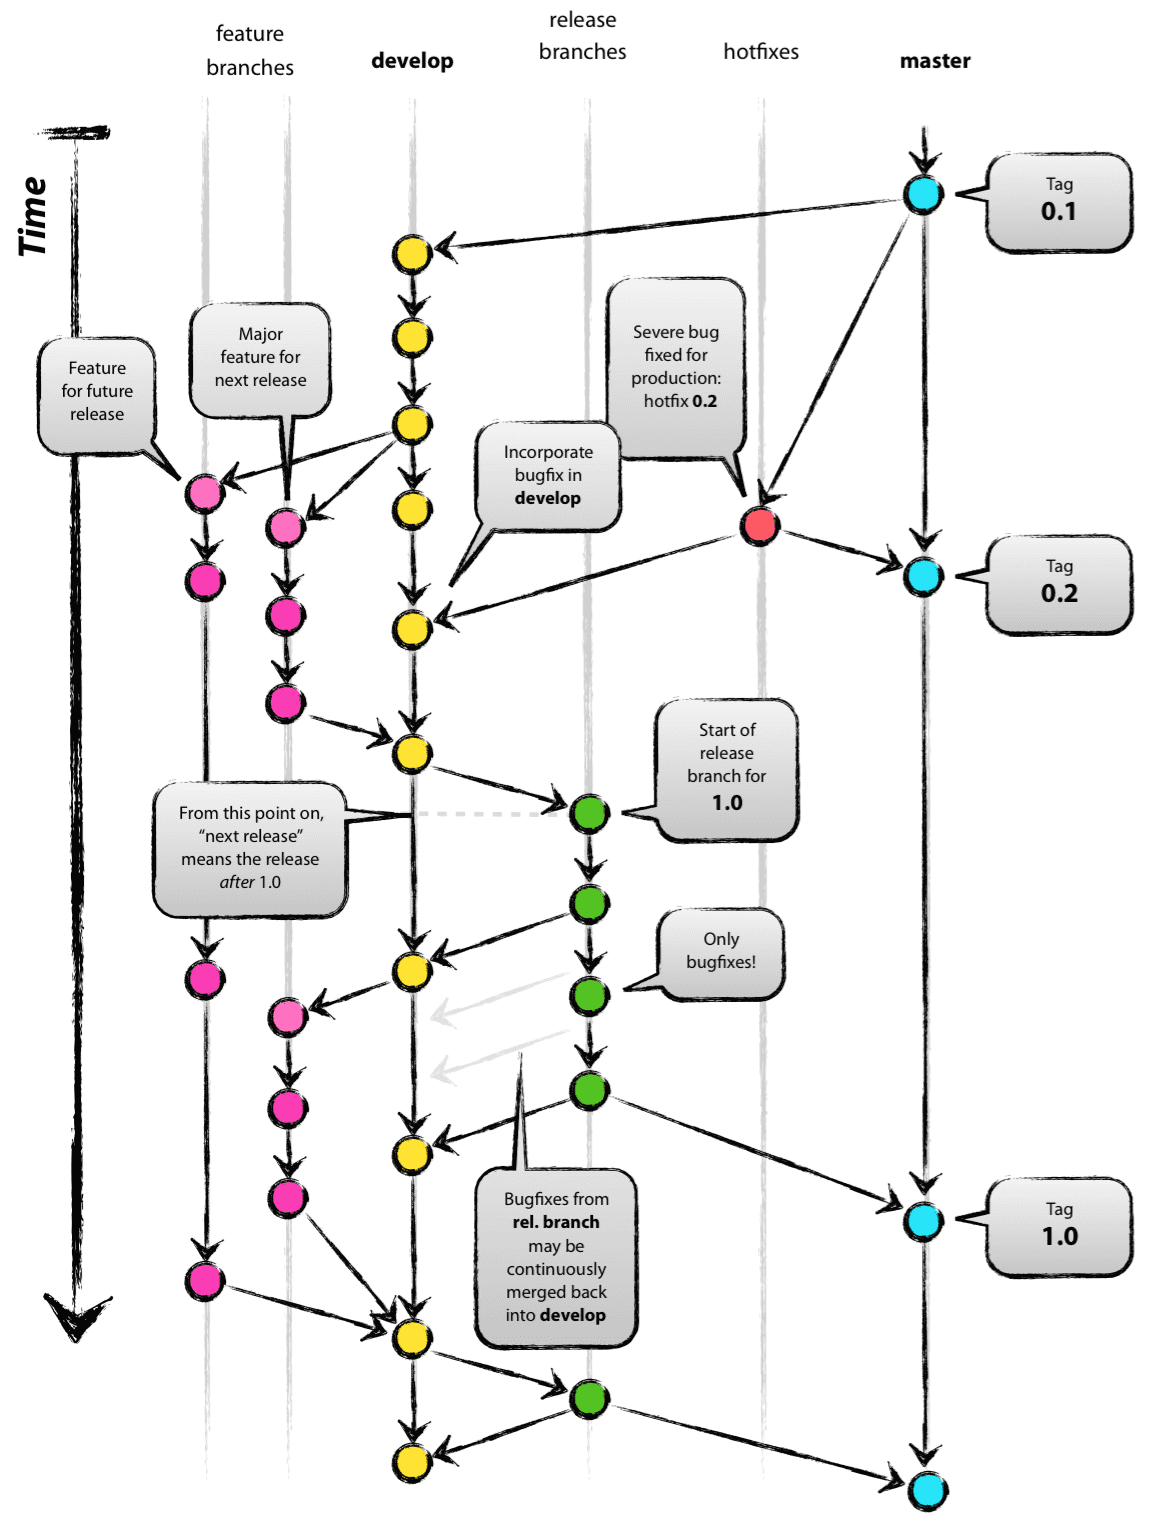
\includegraphics[scale=0.25]{gitflow.png}
		\caption{Styl pracy - Git Flow}
\end{figure}